\section{Financial Economics Tools and Experimental Verifications}
\label{sec:econ}

Section~\ref{sec:evaluation} establishes DeXposure-FM's predictive performance on machine learning benchmarks. We now translate those outputs into financial-economics tools and provide experimental verifications that connect the model's forecasts to macroprudential use cases.

\subsection{Macroprudential Applications}
\label{subsec:macro-applications}

DeXposure-FM generates several outputs directly relevant to macroprudential monitoring of decentralised financial infrastructure, addressing the data gaps highlighted by international standard-setters \citep{FSB2023,IOSCO2023DeFi}.

\subsubsection{Systemic Risk Measurement: SIS and Spillovers}
\label{subsubsec:systemic-risk}
\textbf{Implementation.}
We compute protocol-level and network-level indicators on each weekly exposure snapshot. For protocol $p$, the Systemic Importance Score (SIS) combines interconnectedness, exposure concentration, and scale:
\begin{equation}
\text{SIS}_p = \alpha \cdot \text{PageRank}_p + \beta \cdot \text{TailExposure}_p + \gamma \cdot \log(\text{TVL}_p),
\label{eq:sis}
\end{equation}
where $\text{TailExposure}_p$ is the share of $p$'s top-$k$ outgoing exposures (we use $k=5$), and $\alpha,\beta,\gamma$ are non-negative weights that sum to 1 (default $\alpha=\beta=\gamma=1/3$). In parallel, we aggregate edge weights into a sector-to-sector spillover matrix $\mathbf{S}\in\mathbb{R}^{K\times K}$ where $S_{ij}$ is total exposure from sector $i$ to $j$, and compute a scale-invariant spillover concentration index as the HHI of off-diagonal entries:
\begin{equation}
\text{SpilloverIndex} = \text{HHI}\left(\{S_{ij} : i \neq j\}\right).
\end{equation}
\textbf{Use case.}
These measures operationalise the network-theoretic insight that interconnectedness, not just size, determines systemic fragility \citep{Acemoglu2015SystemicRisk,GlassermanYoung2016Contagion}. Weekly SIS rankings help identify protocols whose distress would propagate broadly, while spillover monitoring highlights sector pairs that act as risk conduits (e.g., stablecoins and bridges) \citep{KosseEtAl2023Stablecoin,ESRB2025,DieboldYilmaz2012}.

\subsubsection{Stress Testing and Contagion Assessment}
\label{subsubsec:contagion}
\textbf{Implementation.}
We implement a DebtRank-style contagion simulation to assess systemic loss propagation, following the loss-allocation logic of \cite{EisenbergNoe2001} and \cite{BattistonEtAl2012DebtRank}. Given an initial shock to protocol $p_0$ with loss ratio $\delta_0$:
\begin{enumerate}
  \item \textbf{Initialize:} $\text{Loss}_{p_0} = \delta_0 \cdot \text{TVL}_{p_0}$.
  \item \textbf{Propagate:} When a distressed debtor $p$ has loss $\text{Loss}_p$, we allocate its loss to its creditors $q$ proportionally to their exposures $E_{qp}$:
  \begin{equation}
    \Delta \text{Loss}_q \;=\; \text{Loss}_p \cdot \frac{E_{qp}}{\sum_{q'} E_{q'p}}.
  \end{equation}
  \item \textbf{Iterate:} If $\text{Loss}_q > \tau \cdot \text{TVL}_q$ (distress threshold $\tau=0.1$), protocol $q$ becomes distressed and propagates losses to its creditors. Losses are capped at $\text{TVL}_q$.
  \item \textbf{Terminate:} When no new protocols become distressed.
\end{enumerate}
We report total system loss (as a percentage of total TVL), contagion depth (propagation rounds), and affected-protocol counts. The three stress scenarios used throughout are: top protocol shock (50\% TVL loss), top-5 protocols shock (30\%), and bridge sector shock (100\%).

\textbf{Empirical verification.}
Section~\ref{subsec:stability} evaluates \emph{forward-looking} stress testing: we run the same simulator on $G_t$ (persistence baseline), $\hat{G}_{t+h}$ (model forecast), and $G_{t+h}$ (realized future) and compare the resulting system losses. Although persistence is hard to beat on average due to high edge overlap, DeXposure-FM improves in the worst 20\% tail regime where persistence fails (Table~\ref{tab:contagion-advantage}), with gains concentrated in bridge-sector shocks (Figure~\ref{fig:contagion-advantage}). Operationally, this suggests using the foundation model as a \emph{backstop} for scenario analysis during non-stationary periods.

\subsubsection{Forward-looking Risk Metric Forecasting}
\label{subsubsec:forward-looking-risk}
\textbf{Implementation.}
Beyond stress testing, we can forecast aggregate stability indicators by first predicting a future exposure graph $\hat{G}_{t+h}$ and then computing deterministic risk metrics on it (e.g., TVL concentration, edge concentration, network density, spillover index, and summary statistics of SIS). We compare these predicted metrics to their realized counterparts on $G_{t+h}$ across the 2025 hold-out set.

\textbf{Empirical verification.}
Figure~\ref{fig:forward-risk-scatter} reports predicted vs.\ realized risk metrics for $h\in\{1,4,8,12\}$. As expected under strong network persistence, many aggregates are difficult to outperform with persistence-style baselines, but the forecasts remain useful for \emph{trend monitoring} and for triggering deeper scenario analysis when predicted metrics move sharply.

\begin{figure}[t]
\centering
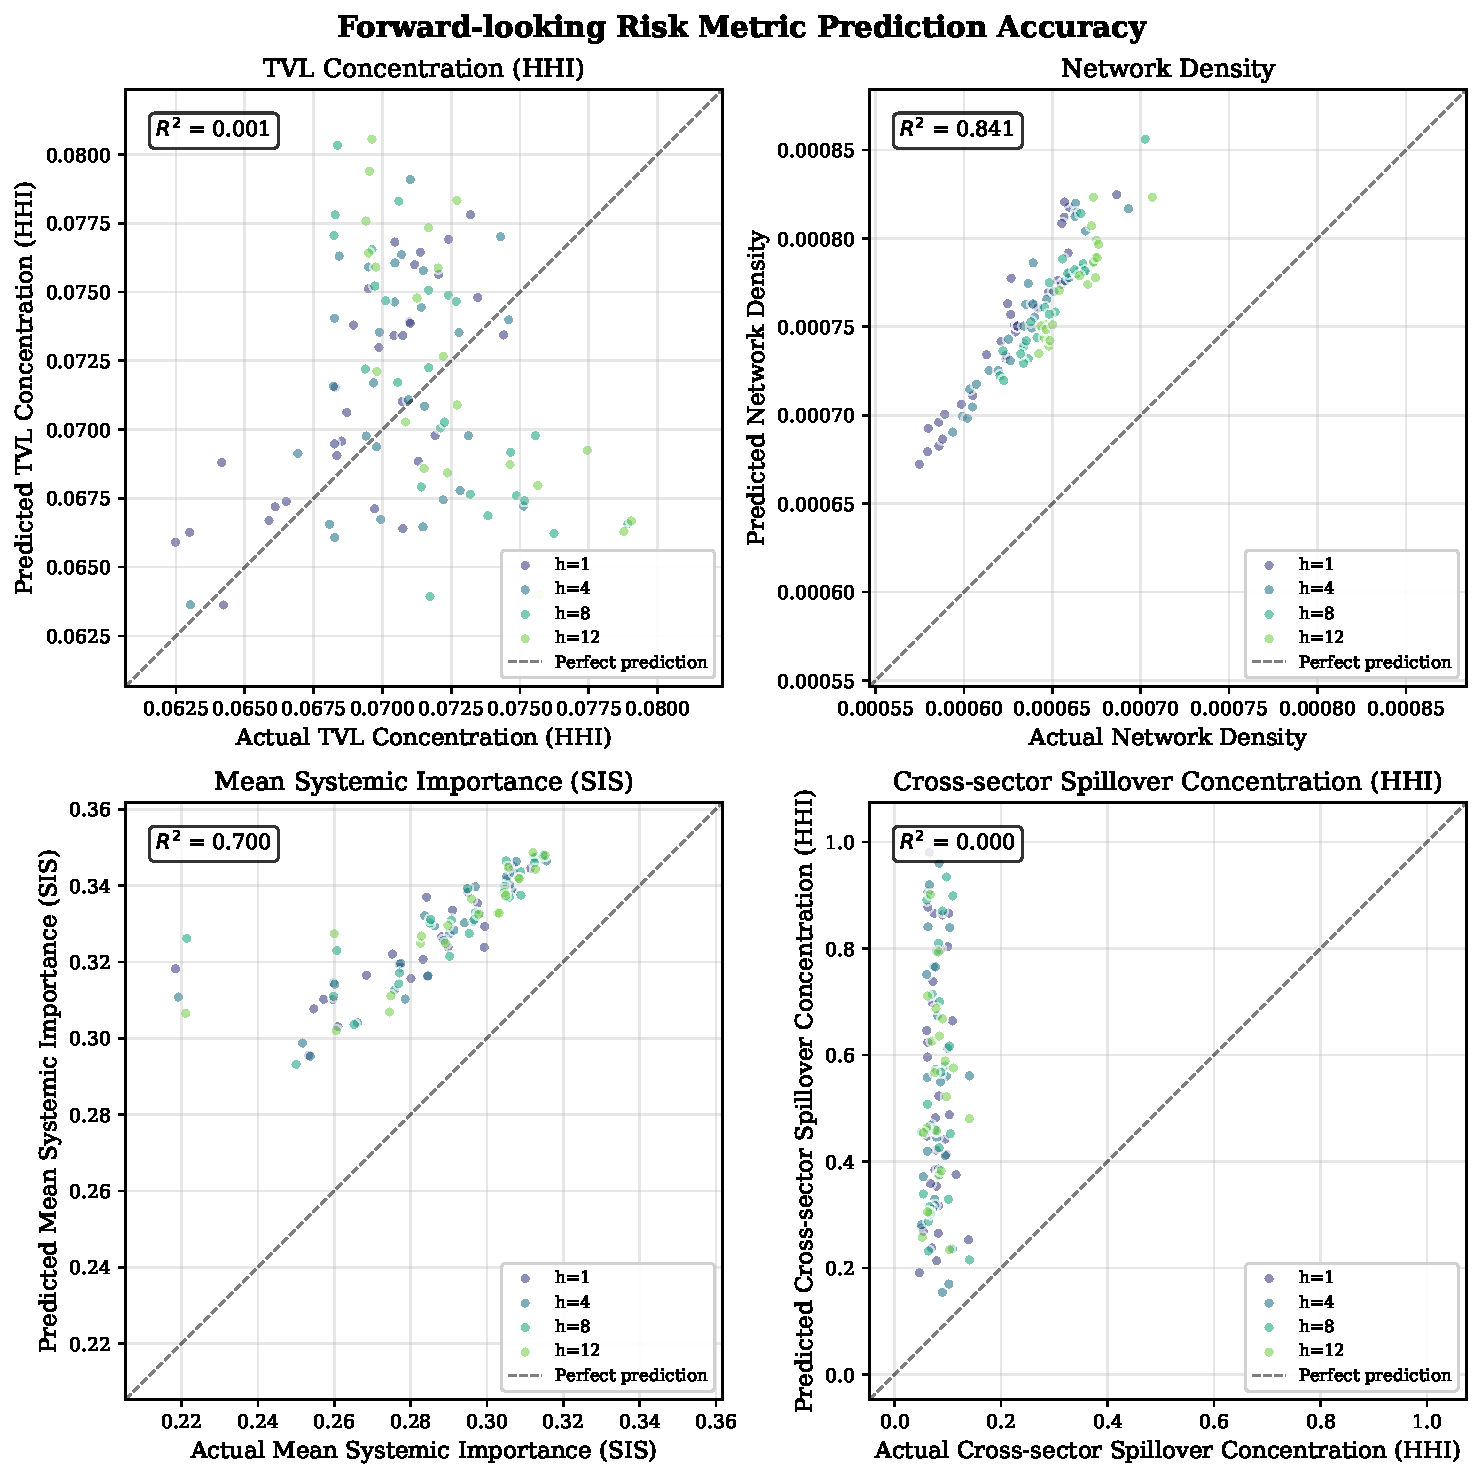
\includegraphics[width=0.95\textwidth]{figures/fig_forward_risk_scatter.pdf}
\caption{Forward-looking risk metric forecasting on predicted exposure graphs. Each point compares a realized metric on $G_{t+h}$ (x-axis) to the same metric computed on the predicted graph $\hat{G}_{t+h}$ (y-axis), across horizons.}
\label{fig:forward-risk-scatter}
\end{figure}

\subsubsection{Early Warning Signals and Event Studies}
\label{subsubsec:shock-events}
\textbf{Implementation.}
We examine two major stress events: the Terra/Luna collapse (May 9, 2022) and the FTX collapse (November 7, 2022). To avoid event leakage, for each event we train an event-specific forecaster using only snapshots strictly prior to the event window, then generate one-step-ahead forecasts within the event window. We track structural indicators and stress-test outcomes (via Section~\ref{subsubsec:contagion}) and monitor potential early warning features:
\begin{itemize}
  \item Density change: $\Delta\rho_t = (\rho_t - \rho_{t-1})/\rho_{t-1}$,
  \item Concentration spikes: $\Delta\text{HHI}_t > 2\sigma$,
  \item Assortativity shifts: rapid changes in degree correlation.
\end{itemize}

\textbf{Empirical verification.}
Table~\ref{tab:shock-results} summarizes structural shifts during the event windows, and Figure~\ref{fig:early-warning} compares predicted vs.\ realized trajectories for risk concentration and stress-test loss. These case studies illustrate how model-based forecasting can complement descriptive monitoring by providing forward-looking alerts around regime changes.

\begin{table}[t]
\centering
\small
\begin{tabular}{lcccc}
\hline
\textbf{Event} & \textbf{Pre-TVL (\$B)} & \textbf{Post-TVL (\$B)} & \textbf{$\Delta$TVL} & \textbf{$\Delta$Edges} \\
\hline
Terra/Luna & 257.1 & 171.0 & $-$33.5\% & +9.4\% \\
FTX & 127.0 & 177.2 & +39.5\% & $-$3.3\% \\
\hline
\end{tabular}
\caption{Network structure changes during stress events. Terra/Luna shows a classic flight-to-quality pattern with TVL collapse but edge count increase as capital reorganizes across protocols. The FTX event shows a \emph{positive} $\Delta$TVL because our dataset captures only on-chain DeFi protocols: the collapse of a centralised exchange triggered capital migration \emph{into} DeFi as users withdrew funds to self-custody, consistent with the ``flight to decentralisation'' narrative \citep{VidalTomasEtAl2023FTX}.}
\label{tab:shock-results}
\end{table}

\begin{figure}[t]
\centering
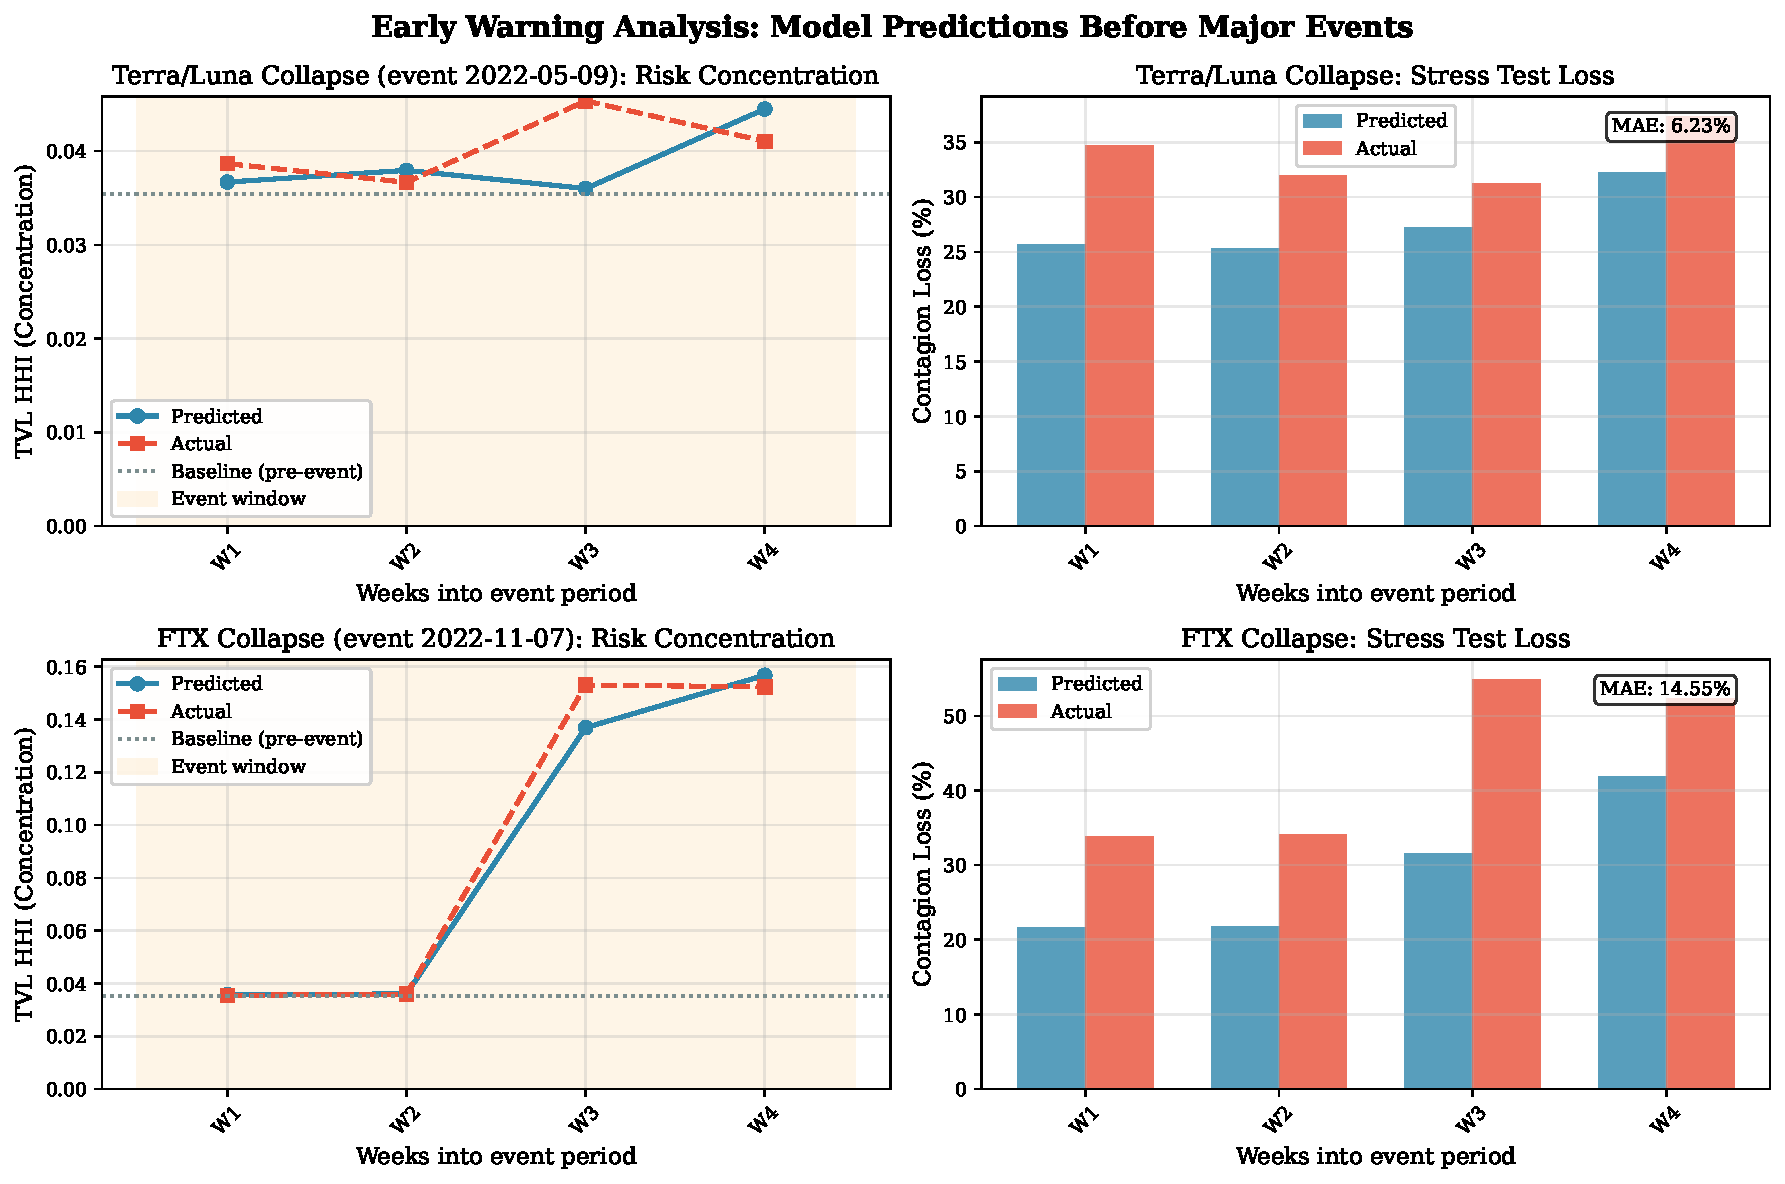
\includegraphics[width=0.95\textwidth]{figures/fig_early_warning.pdf}
\caption{Early warning event studies. For each event window, we compare predicted vs.\ realized risk concentration (HHI) and predictive stress-test loss (contagion system loss \%).}
\label{fig:early-warning}
\end{figure}


\subsection{Validity and Scope}
\label{subsec:validity}

Model-based risk measures are only as reliable as the conditions under which they were trained and validated \citep{MullainathanSpiess2017}. We identify several boundaries that users should keep in mind.

\paragraph{Stable versus turbulent regimes.}
The DeXposure dataset exhibits 98.5\% mean edge overlap week-to-week, meaning most credit relationships persist. Under such stable conditions, edge-existence forecasting is highly accurate (DeXposure-FM AUROC 0.993 at $h=12$; Table~\ref{tab:main-results}). During structural breaks---new protocol launches, governance attacks, or rapid deleveraging---the historical edge distribution may shift abruptly. In these regimes, persistence-style baselines can fail, and forward-looking models can add the most value (e.g., the worst20\% tail-regime gains in Table~\ref{tab:contagion-advantage}).

\paragraph{Coverage.}
DeXposure-FM is trained exclusively on on-chain DeFi protocols sourced from DeFiLlama. It does not observe:
\begin{itemize}
  \item Centralised exchange (CEX) balances or order-book exposures,
  \item Over-the-counter (OTC) derivatives or lending agreements,
  \item Off-chain reserves backing stablecoins (e.g., Treasury holdings of USDC) \citep{AnaduEtAl2023StablecoinsMMF}.
\end{itemize}
Consequently, the model captures intra-DeFi contagion but cannot directly assess spillovers to or from traditional financial institutions---a gap that matters as DeFi-TradFi linkages deepen \citep{ESRB2025}.

\paragraph{Temporal resolution.}
The dataset aggregates to weekly snapshots. Intraday or even daily dynamics---such as flash-loan attacks \citep{Qin2021FlashLoans} or rapid liquidation cascades \citep{Warmuz2023ToxicLiquidationSpirals}---are smoothed out. For high-frequency risk monitoring, complementary tools operating on block-level data would be required.


\subsection{Practical Caveats for Policymakers}
\label{subsec:caveats}

\paragraph{Complement, not replace, qualitative judgment.}
Model outputs such as SIS rankings and spillover indices are quantitative summaries, not definitive verdicts. A protocol may rank low on SIS yet pose idiosyncratic risks (e.g., smart-contract vulnerabilities, oracle manipulation) that network topology alone cannot capture \citep{DuleyEtAl2023Oracle,Gogol2024SoKDeFi}. Supervisors should triangulate model signals with code audits, governance analyses, and market intelligence.

\paragraph{TVL as a proxy for exposure.}
Total Value Locked is a convenient but imperfect measure \citep{Bertomeu2024}. It aggregates heterogeneous assets---stablecoins, volatile tokens, LP positions---without adjusting for liquidity or collateralisation quality. A protocol with \$1B in illiquid governance tokens is not equivalent to one with \$1B in USDC. Future work could incorporate asset-level risk weights to refine exposure estimates.

\paragraph{Model drift and retraining.}
DeFi evolves rapidly: new chains launch, token standards change, and incentive mechanisms shift. A model trained on 2020--2024 data may gradually lose accuracy as the ecosystem diverges from historical patterns. Periodic retraining on updated snapshots is essential to maintain forecast quality.

\paragraph{Cross-chain data consistency.}
DeXposure aggregates data across 602 blockchains, each with its own indexing quirks and oracle delays. Minor inconsistencies in timestamp alignment or token-price feeds can introduce noise. Users should be aware that edge weights near reporting boundaries may reflect data artefacts rather than genuine exposure changes.
